
% Explicar:
% - objectivos das experiencias
% - eventuais métricas de desempenho
% - condições experimentais (ambiente hospitalar, fig 5.1, etc.)
% - quaisquer eventuais parameterizações importantes no contexto específico dos trials
% - resultados e discussão

After developing and analyzing the different \acs{IoT} system components, it is time to evaluate its overall performance in a real-world scenario. In this chapter, the results of the trials performed on the overall \acs{IoT} system are presented and discussed. 

\paragraph{} 

\section{Hospital Pilot}

For the hospital trial, the proposed \acs{IoT} system has been deployed in a clinical facility within Centro Hospitalar e Universitário de Coimbra (CHUC), during which two volunteers have been continuously monitored using the system. A \textit{Smart box}, one \textit{Biosticker} and one oximeter are assigned to each volunteer for the duration of the trial. The oximeter is attached to the patient's right-hand index finger recording pulse oximeter data and the \textit{Biosticker} is attached to the patient's chest recording the other biosignals (body temperature, \acs{ECG}, etc., as discussed in Section \ref{sec:biosticker_data}). The patients remained in bed for the entirety of the trial, always keeping the \textit{Smart box} at most 5 meters away from the patient, as shown in Figure \ref{fig:hospital-trial}. The Wi-Fi network used to connect the \textit{Smart box} to the \textit{Smart Gateway} has been provided by the hospital IT, and is also being used concurrently by the researchers during the study. Additionally, each device is assigned a fixed \acs{IP} to facilitate the deployment of the infrastructure, and ensure the devices are able to communicate with one another at all times.

\paragraph{} The acquisition rates of the sensors are as defined in Section \ref{chap:smartbox}. As mentioned in the previous chapter, for this first trial, the subscription rates for the \acs{FHIR} communications have been previously established, corresponding to 1 minute intervals for all sensors, \textit{i.e.} the latest measurement of each biosignal is communicated every minute to the \acs{HIS}.

\begin{figure}[H]
    \centering
    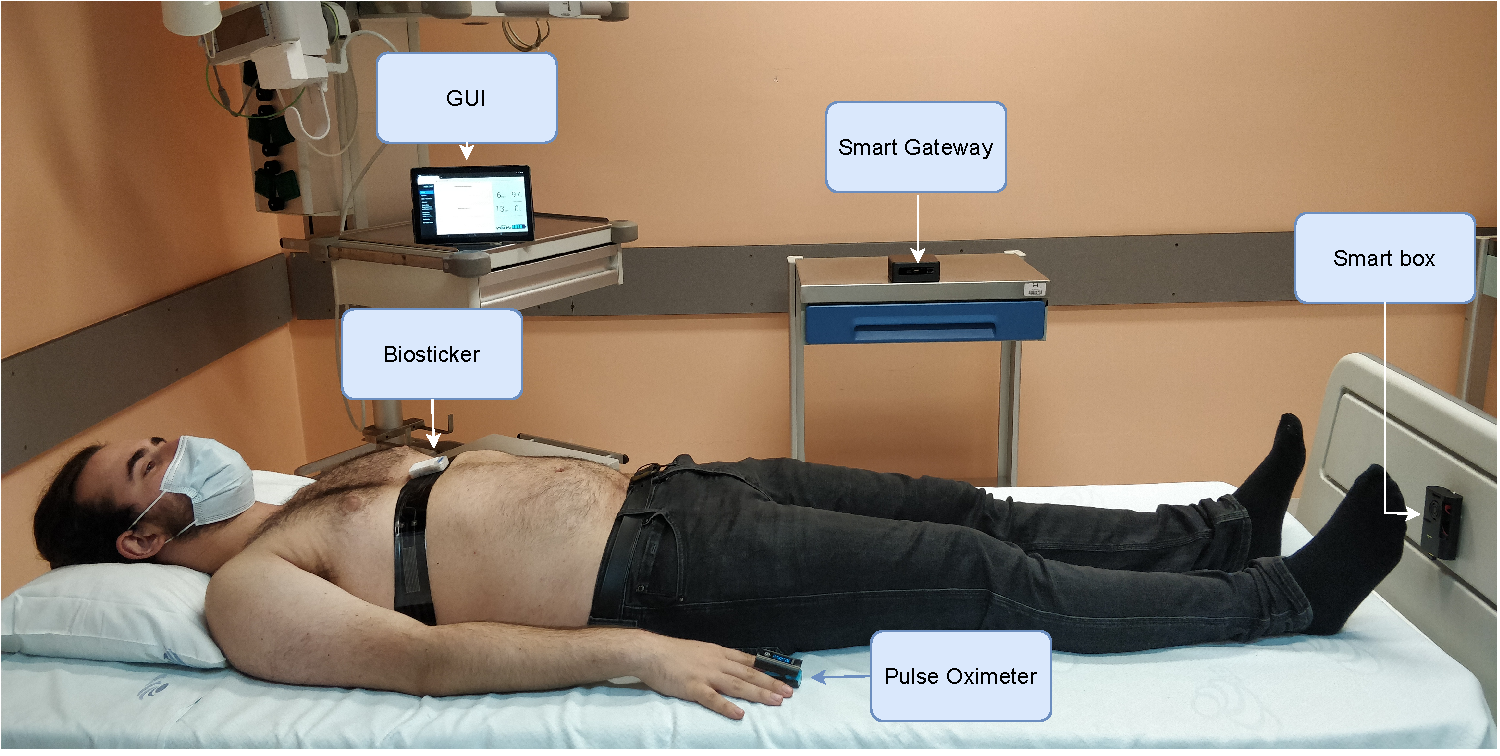
\includegraphics[width=\linewidth]{images/hospital-trial-setup.pdf}
    \caption[Conceptual illustration of the system components within a medical facility.]{Conceptual illustration of the system components within a medical facility.}
    \label{fig:hospital-trial}
\end{figure}

In this trial, the objective is to evaluate the stability and reliability of the infrastructure in a real-world scenario. To this end, the bandwidth used by the \acs{MQTT} and \acs{FHIR} communication protocols are analyzed to evaluate the reliability of the system, in order to check for interruptions of the communication and observe if there are any issues with the communication; and the system resource usage (\acs{CPU} and \acs{RAM}) is also monitored to evaluate the system's stability. To evaluate the performance of the proposed system, the following performance metrics were defined and measured throughout the tests:

\begin{itemize}
    \item \acs{MQTT} bandwidth -- Rate of data exchanged between all \textit{Smart boxes} and \textit{Smart Gateway};
    \item \acs{FHIR} bandwidth -- Rate of data exchanged between the \textit{Smart Gateway} and \acs{HIS};
    \item Resource usage of \textit{Gateway} services -- \acs{CPU} and \acs{RAM} usage of each \textit{Gateway} service;
\end{itemize}

In the next section, 2 hours of continuous monitorization tests are analyzed and discussed. 

\subsection{Results and Discussion}

Figure \ref{fig:labtest-mqtt-payload-sizes} shows a boxplot of the \acs{MQTT} payload sizes for each type of biosignal message. The deviation in the payload lengths is caused by variations of the number of digits in the numeric entries sent in the messages (\textit{e.g.} acceleration or gyroscope values in the \acs{IMU}), which should result in using more or less characters when the data is serialized into the \acs{JSON} payloads sent to the \acs{MQTT} broker. For the heart rate, respiration rate and pulse oximetry messages, due to the nature of these biosignals the number of digits does not change, so the payload size remains constant throughout the tests. Taking this information into account, together with the acquisition rate for each biosignal as defined in Section \ref{chap:smartbox}, the estimated bandwidth is expected to be close to $ 21.96 \pm 0.02$ kbps.

\begin{figure}[H]
    \centering
    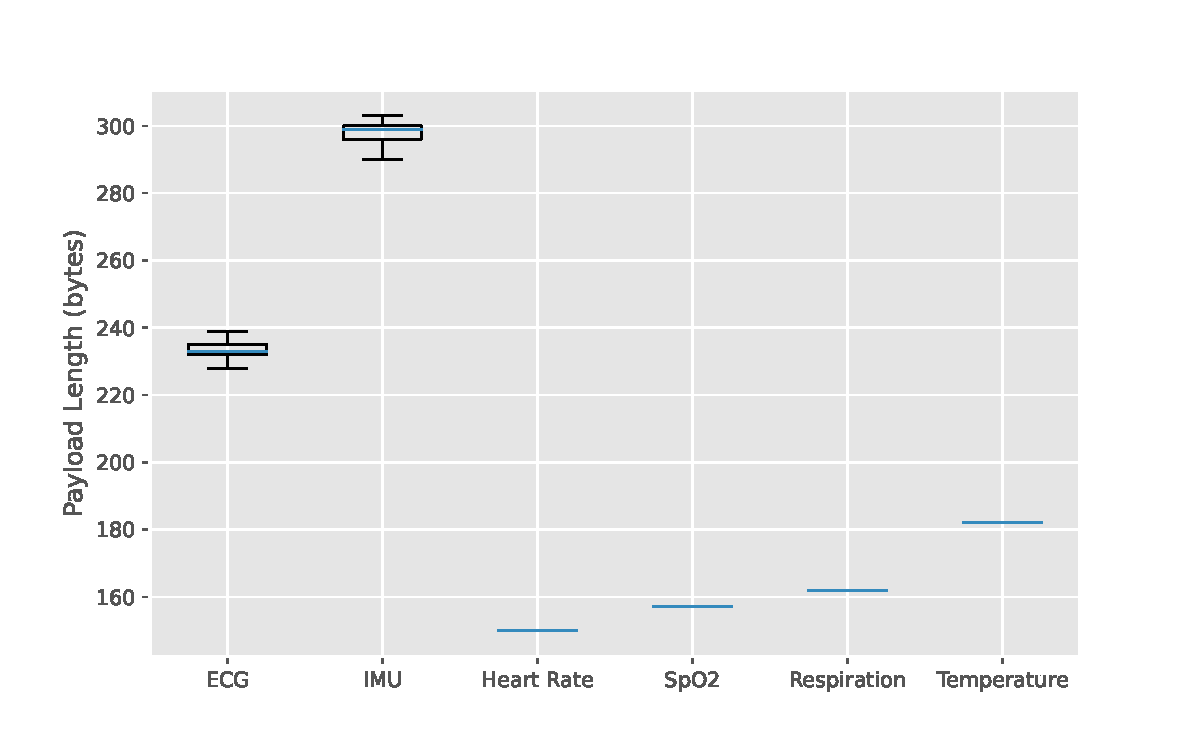
\includegraphics[width=0.85\linewidth]{images/labtest_mqtt_payload_sizes.pdf}
    \caption{\acs{MQTT} payload sizes measured for each type of biosignal sensor message during the hospital trial.}
    \label{fig:labtest-mqtt-payload-sizes}
\end{figure}

The following graphs have been obtained using the data collected in the hospital trial using 2 \textit{Smart boxes} and 1 \textit{Smart Gateway}. Figure \ref{fig:pilot-mqtt-bandwidth} and \ref{fig:pilot-fhir-bandwidth} show the measured \acs{MQTT} and \acs{FHIR} bandwidth respectively, averaged over 1 min.  Figure \ref{fig:pilot-cpu-usage} and \ref{fig:pilot-ram-usage} show the measured \acs{CPU} and \acs{RAM} usage.

\begin{figure}[H]
    \begin{minipage}{0.49\linewidth}
        \centering
        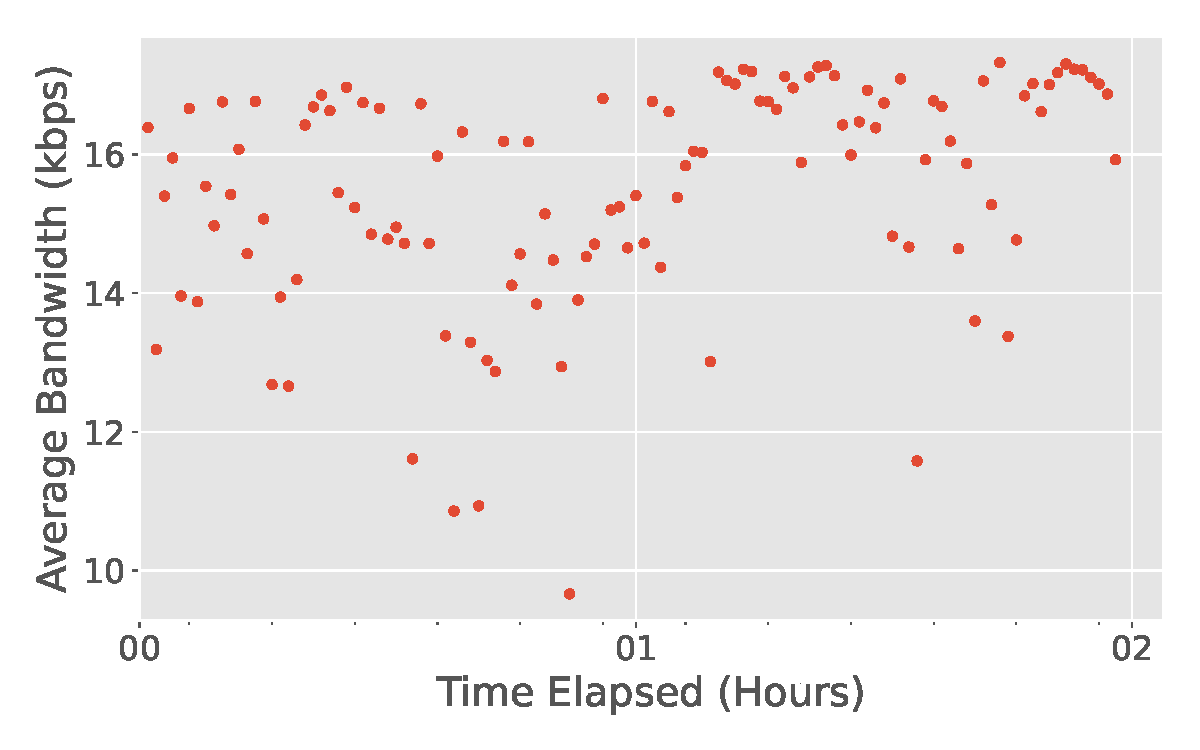
\includegraphics[width=\linewidth]{images/pilot_mqtt_bandwidth.pdf}
        \caption{Average \acs{MQTT} bandwidth usage measured over time during the hospital trial. }
        \label{fig:pilot-mqtt-bandwidth}
    \end{minipage}
    \hspace{0.02\linewidth}
    \begin{minipage}{0.49\linewidth}
        \centering
        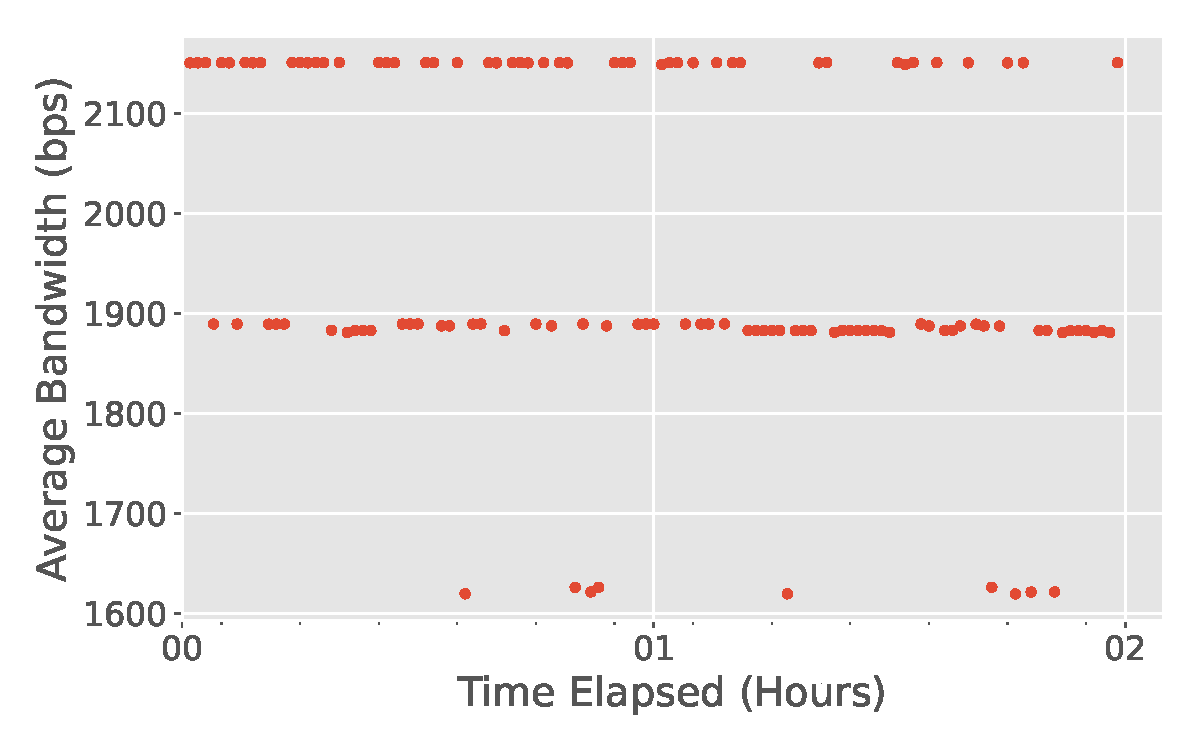
\includegraphics[width=\linewidth]{images/pilot_fhir_bandwidth.pdf}
        \caption{Average \acs{FHIR} bandwidth usage measured over time during the hospital trial.}
        \label{fig:pilot-fhir-bandwidth}
    \end{minipage}
\end{figure}


\paragraph{} Yet, the measured bandwidth data is very different from the abovementioned value -- with an average value of $15.513 \pm 1.605$ kbps. Not only it is ${\sim}  30\%$ lower than the estimated value, the bandwidth results are very sparse as seen by the standard deviation of 1.605 kbps, which corresponds roughly to 10 messages per second. Despite our efforts, it is not possible to determine the exact nature of this deviation since there are no records of the \acs{MQTT} transmissions on the \textit{Smart box} side. 

There are several factors which influence the \acs{MQTT} bandwidth, any of which (or combination of which) could be causing this issue:

\begin{itemize}
    \item The custom \textit{Mosquitto} plugin intercepts messages to authenticate and validate the \textit{Smart boxes}. This introduces an additional processing delay that could impact the measured bandwidth.
    \item The \textit{Smart boxes} continuously receive data from the \textit{Biostickers}, so any interruption on the communication between these devices inevitably would reduce the amount of messages sent. During the hospital trial, numerous \acs{BLE} connection issues were reported, so this is likely one of the main causes for the observed variance.
    \item Since the \textit{Smart boxes} are connected using Wi-Fi, and since the network was being actively used by researchers throughout the trials, there could be fluctuations in the transmission of the data caused by network constraints. This could contribute to the issue at hand, but should not be significant enough to take into account.
\end{itemize}

\paragraph{} Due to these irregularities, the \acs{FHIR} bandwidth is impacted, as seen in Figure \ref{fig:pilot-fhir-bandwidth}. The graph shows the data arranged in different ``levels'', each corresponding to the successful transmission of a certain amount of messages. These levels are discretized as the subscriptions are only triggered once a minute. In this case, the maximum level (at ${\sim}  270$ bps) corresponds to sending all messages in that minute, ${\sim}  240$ bps when one message is not sent in that minute, and ${\sim}  200$ bps when two messages are not sent instead. The messages are not being sent because there is no new information in the data storage, which may be caused by the issues previously referred. Additionally, all messages sent by the \textit{Smart Gateway} to GlobalCare \acs{HIS} have been confirmed on the \acs{HIS} side as well, thus validating the \acs{FHIR} service developed.  

\paragraph{} Regarding \acs{CPU} and \acs{RAM} usage, it is observed to be very low across all services running on the \textit{Smart Gateway} (the hardware specification can be found on Table \ref{tab:NUCspecification}) with less than 10\% \acs*{CPU} usage and 2\% \acs*{RAM} usage overall, meaning that the service architecture is fairly efficient. This also provides ample resources for deploying additional analytics services locally, instead of relying on cloud services.

\begin{figure}[H]
    \begin{minipage}{0.45\linewidth}
        \centering
        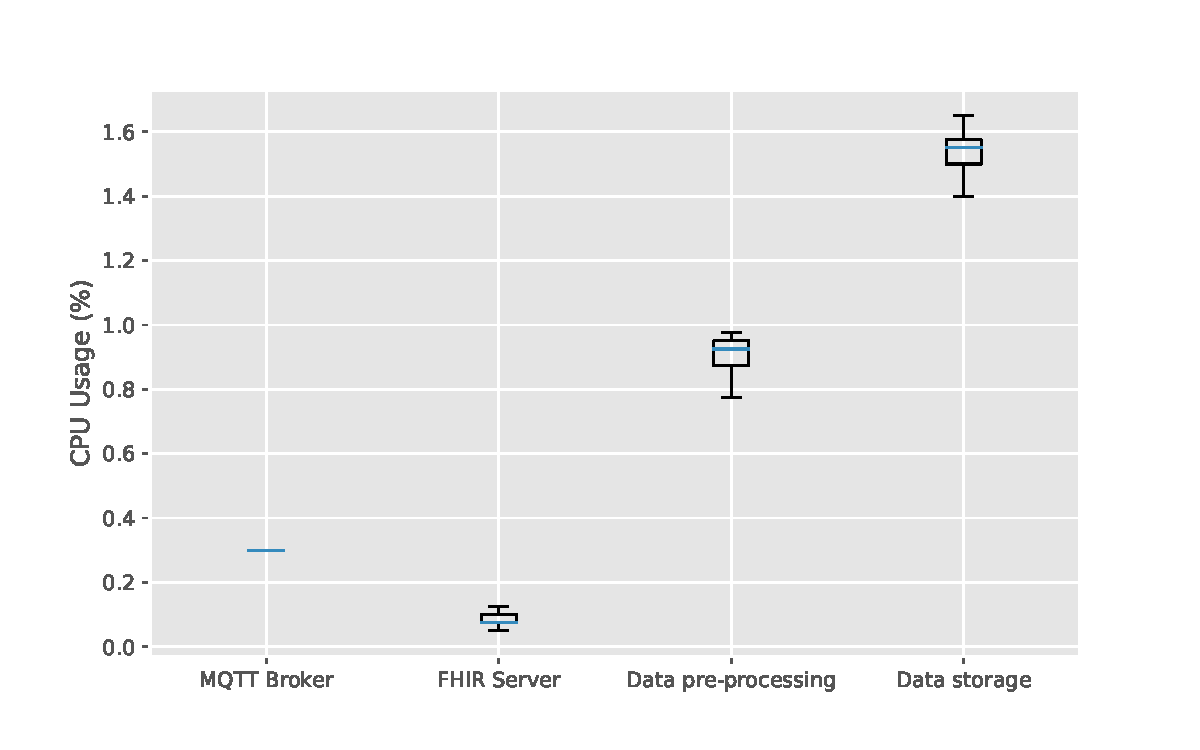
\includegraphics[width=\linewidth]{images/pilot_cpu_usage.pdf}
        \caption{\acs{CPU} usage of each \textit{Smart Gateway} service measured over time during the hospital trial.}
        \label{fig:pilot-cpu-usage}
    \end{minipage}
    \hspace{0.05\linewidth}
    \begin{minipage}{0.45\linewidth}
        \centering
        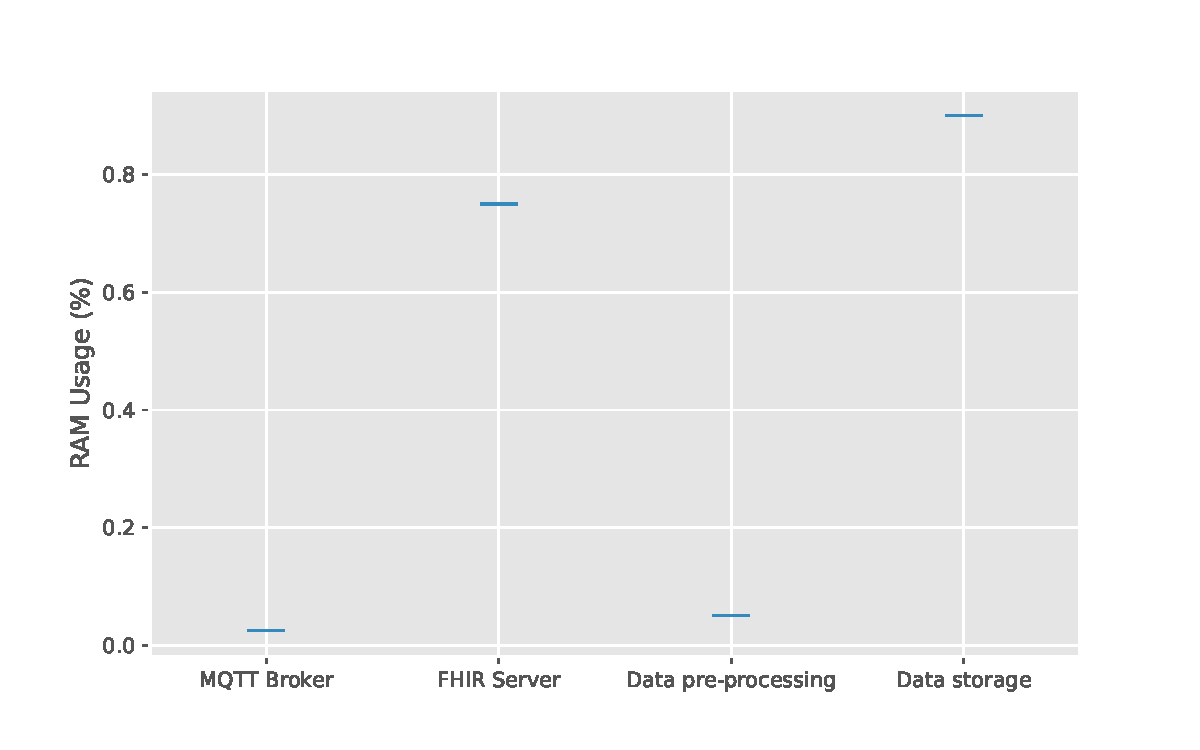
\includegraphics[width=\linewidth]{images/pilot_ram_usage.pdf}
        \caption{\acs{RAM} usage of each \textit{Smart Gateway} service measured over time during the hospital trial.}
        \label{fig:pilot-ram-usage}
    \end{minipage}
\end{figure}



\paragraph{} When analyzing the data of the trial, the latency values for each \textit{Smart box} were observed to be significantly different from one another. This was later determined to have been caused by clock drift\footnote{https://ubuntu.com/server/docs/network-ntp}, as the service used to maintain the system clock updated (which is the default service that is pre-installed in Ubuntu) could not provide sufficient precision when using public \acf{NTP} servers. To solve this, a different strategy is required: the \textit{Smart boxes} must periodically synchronize the system clock directly with the \textit{Smart Gateway}, and the \textit{Smart Gateway} synchronizes its clock with a pool of \acs{NTP} servers. This minimizes the differences between the system clocks of the \textit{Smart Gateway} and the \textit{Smart boxes}, significantly improving the precision of the timestamps (from ${\sim}  100$ ms to ${\sim}  10\ \mu$s). 
To implement this, a \acs{NTP} server has been installed in the \textit{Smart Gateway} as well as a high performance \acs{NTP} client in both the \textit{Smart Gateway} and \textit{Smart boxes}. 
%This strategy does introduce additional time differences when comparing the \textit{Smart boxes} with public \acs{NTP} servers, but these are negligible (${\sim}  10\ \mu$s). 

\paragraph{} Due to all the aforementioned issues, it is not possible to fully assess the performance of the overall system. As such, additional tests in a controlled environment have been performed to overcome the weaknesses of the initial experiments. These are discussed in the next section.

\section{Laboratory Tests}

As mentioned, due to the sparsity of the results obtained in the hospital trial, additional tests in a controlled environment have been performed to fully assess the potential of the system.

\paragraph{} The tests have been formulated based on the results of the hospital trial, also using 2 \textit{Smart boxes} and 1 \textit{Smart Gateway}. Since there were \acs{BLE} connection issues on the \textit{Smart box} reported throughout the hospital trial, for these tests the \textit{Smart boxes} generate simulated data to send via \acs{MQTT}, \textit{i.e.} we remove the uncertainty derived from the Bluetooth acquisition issues from the \textit{Biostickers} to the \textit{Smart boxes}. In these tests, the focus is the evaluation of \acs{MQTT} data transmission, thus the \acs{FHIR} server was not used for these tests. Additionally, to determine if the usage of the custom \textit{Mosquitto} plugin is causing the aforementioned issues, tests have been performed with and without using the authentication plugin. These tests were performed within \acs{ISR} facilities, so the network infrastructure was already provided by the \acs{IT} staff. Once again, all devices had static \acs{IP} addresses to facilitate the deployment and troubleshooting of communication failures.

\paragraph{} To assess the performance of the proposed system, the performance metrics defined in the hospital tests were used once more -- \acs{MQTT} bandwidth, \acs{CPU} and \acs{RAM} resource usage -- as well as:

\begin{itemize} 
    %\item Execution time of \acs{SQL} stored procedures -- Interval of time to execute a stored procedure in the data storage.
    \item \acs{MQTT} packet loss -- Loss of data observed.
    \item \acs{MQTT} latency -- Interval of time between the data collection at each \textit{Smart box} and the reception of data in the \textit{Smart Gateway}.
\end{itemize}


\subsection{Results and Discussion}

The following graphs have been obtained using the data collected in the laboratory tests using 2 \textit{Smart boxes} and 1 \textit{Smart Gateway}. Figure \ref{fig:labtest-mqtt-bandwidth} and \ref{fig:labtest-mqtt-latency} show the measured \acs{MQTT} bandwidth and latency respectively, averaged over 1 minute. 

\begin{figure}[H]
    \begin{minipage}{0.49\linewidth}
        \centering
        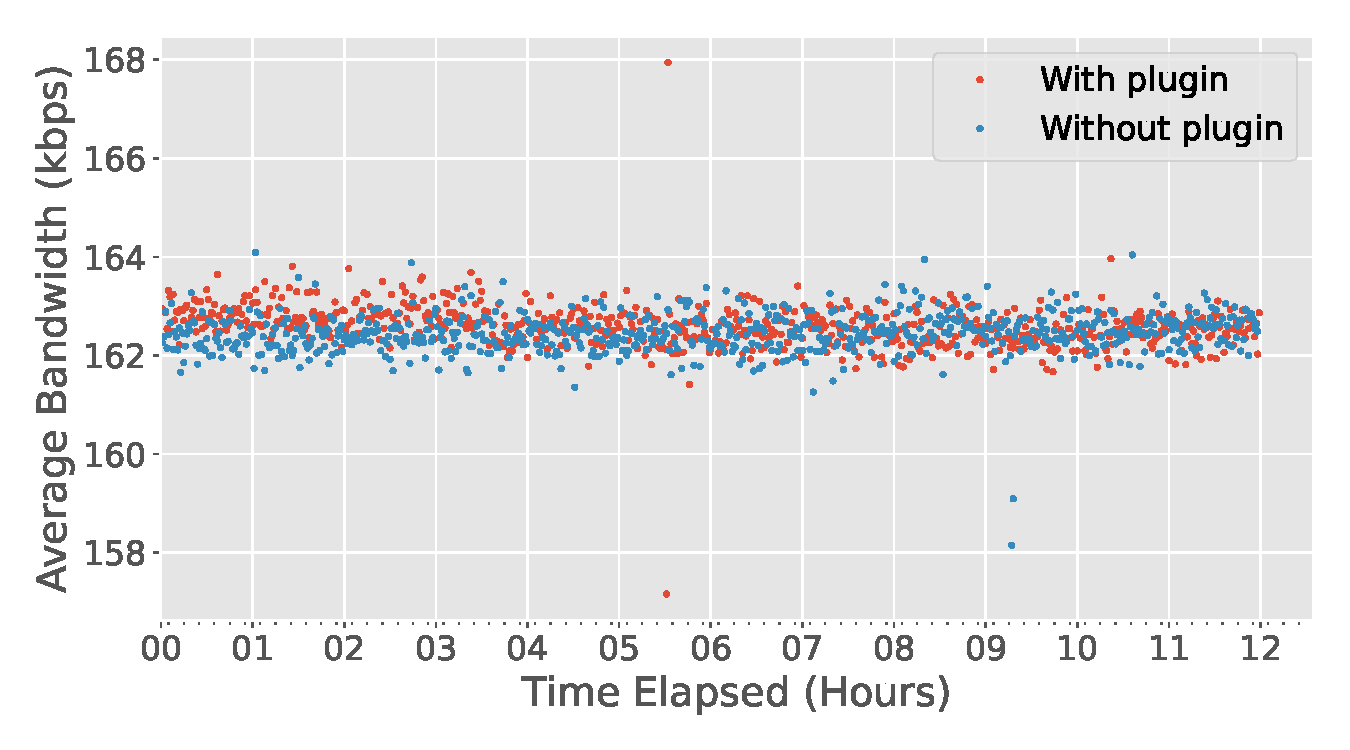
\includegraphics[width=\linewidth]{images/labtest_mqtt_bandwidth.pdf}
        \caption{Average \acs{MQTT} bandwidth usage measured over time during the lab tests.}
        \label{fig:labtest-mqtt-bandwidth}
    \end{minipage}
    \hspace{0.02\linewidth}
    \begin{minipage}{0.49\linewidth}
        \centering
        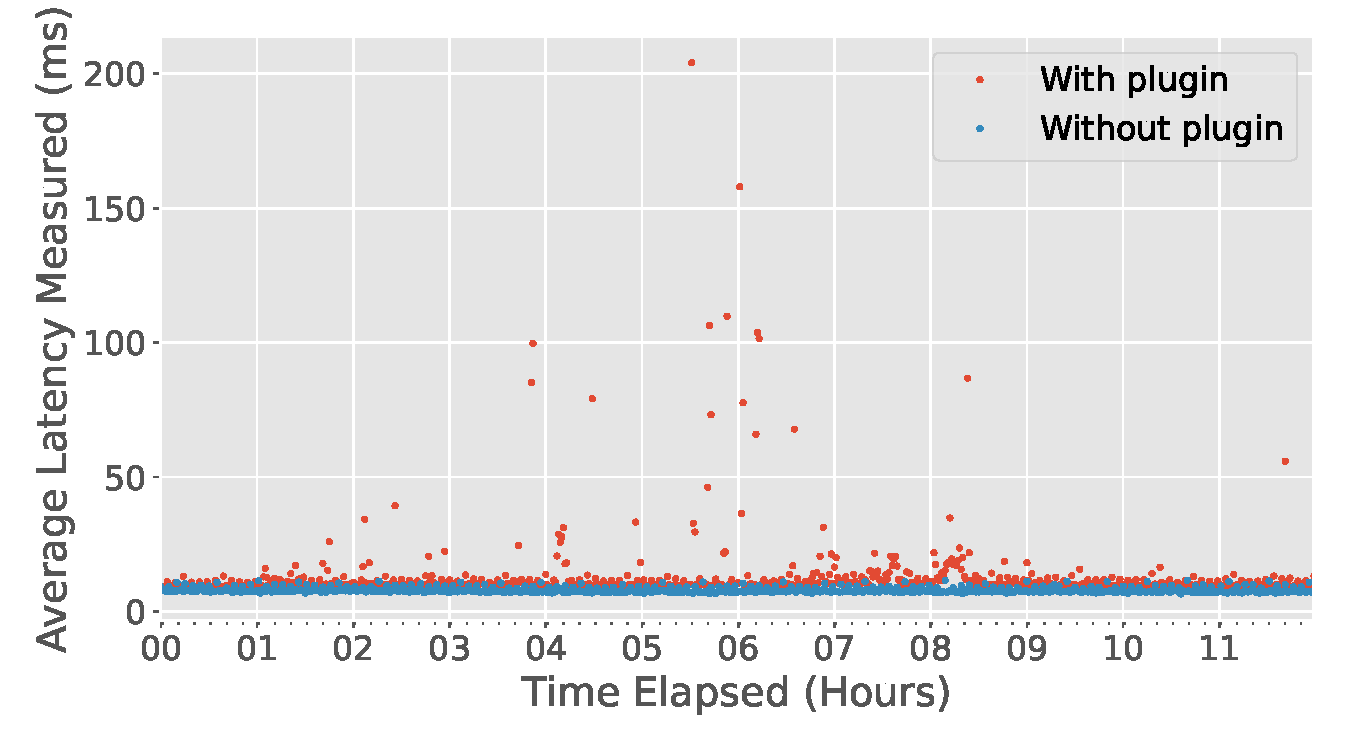
\includegraphics[width=\linewidth]{images/labtest_mqtt_latency.pdf}
        \caption{Average \acs{MQTT} latency measured over time during the lab tests.}
        \label{fig:labtest-mqtt-latency}
    \end{minipage}
    
\end{figure}

As seen in the graphs, the \acs{MQTT} bandwidth is much higher than the value observed in the hospital trials, but still somewhat below the expected value (21.96 kbps). 
This is because the delay caused by the \acs{MQTT} transmission itself was not accounted for, reducing the transmission rate of the simulated sensors very slightly, which translates into a minor difference in the overall \acs{MQTT} bandwidth. Nonetheless, it displays much better results with an average bandwidth of $20.32 \pm 0.06$ kbps using the plugin and $20.31 \pm 0.05$ kbps without using the plugin. Despite this final result seemingly favoring the usage of the plugin, it should be noted that the difference between these values is not statistically significant, and thus can be safely disregarded. It means however that the usage of the plugin does not meaningfully impact the performance of the \acs{MQTT} communications, while also providing authentication and authorization features to the broker.

\paragraph{} One thing to note is that the average latency does show a significant increase ($13.22 \pm 14.07$ ms when using the plugin to $7.86 \pm 0.98$ ms without it), which is expected since the plugin adds a fixed processing delay caused by the requests to the data storage service. However, the latency obtained using the plugin seems to be very sparse (as seen with a standard deviation larger than the latency value itself), which would indicate some sort of data loss, but this is not the case. A full analysis revealed that \textbf{100\%} of the data generated by the \textit{Smart boxes} in this test was captured by the \textit{Smart Gateway}. This means that this delay is being compensated somehow, or that is caused by something else, for example, an issue with the recently introduced \acs{NTP} server, and so it should be researched further. One thing is clear however, and that is that the data is being successfully transmitted and received using \acs{MQTT}. 

\paragraph{} Figure \ref{fig:labtest-ram-usage}, \ref{fig:labtest-ram-usage-noplug}, \ref{fig:labtest-cpu-usage} and \ref{fig:labtest-cpu-usage-noplug} show the measured \acs{RAM} and \acs{CPU} usage, with and without the custom authentication plugin. These values are consistent with those observed in the hospital trials. It is observed that the \acs{CPU} usage of the data storage nearly doubles when using the plugin, which is expected since the plugin performs requests to the data storage whenever a message is received, effectively doubling the amount of requests performed on the data storage -- one request on the plugin to check if the \textit{Smart box} is authorized, one request on the data pre-processing service to store the received data.

\begin{figure}[H]
    \begin{minipage}{0.45\linewidth}
        \centering
        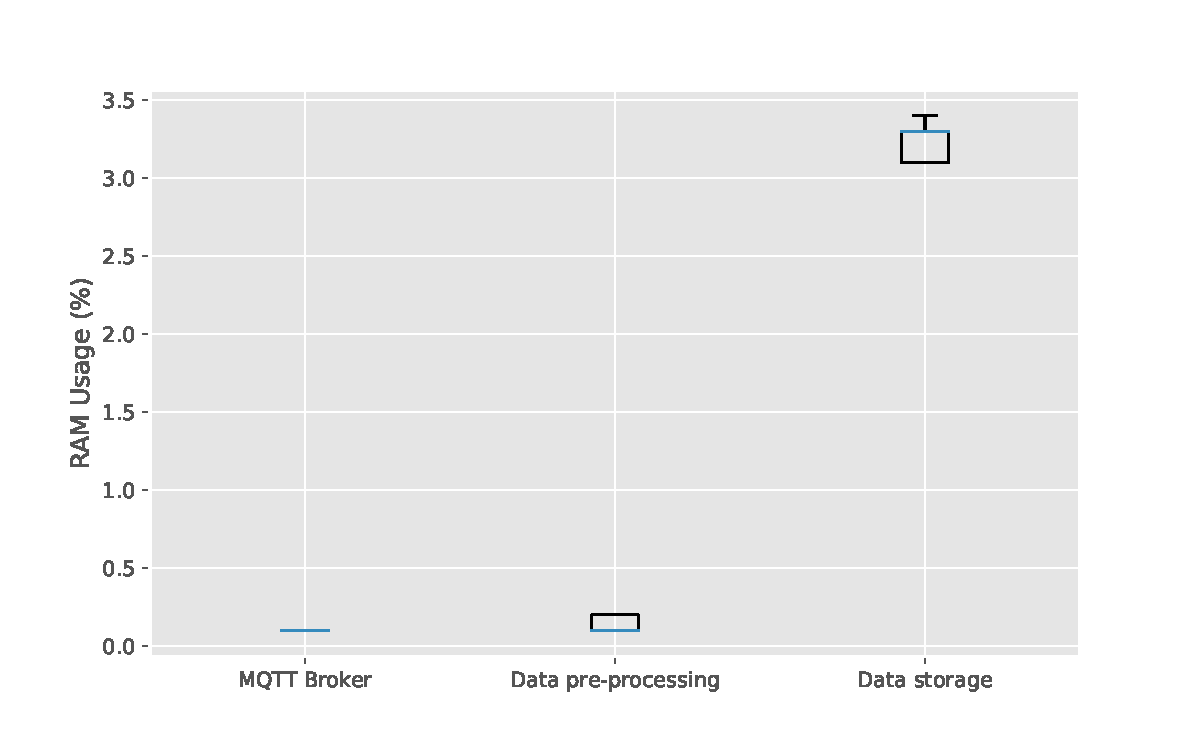
\includegraphics[width=\linewidth]{images/labtest_ram_usage_with_plugin.pdf}
        \caption{Average \acs{RAM} usage of each \textit{Smart Gateway} service measured over time during the lab tests, when using the custom plugin for Mosquitto.}
        \label{fig:labtest-ram-usage}
    \end{minipage}
    \hspace{0.05\linewidth}
    \begin{minipage}{0.45\linewidth}
        \centering
        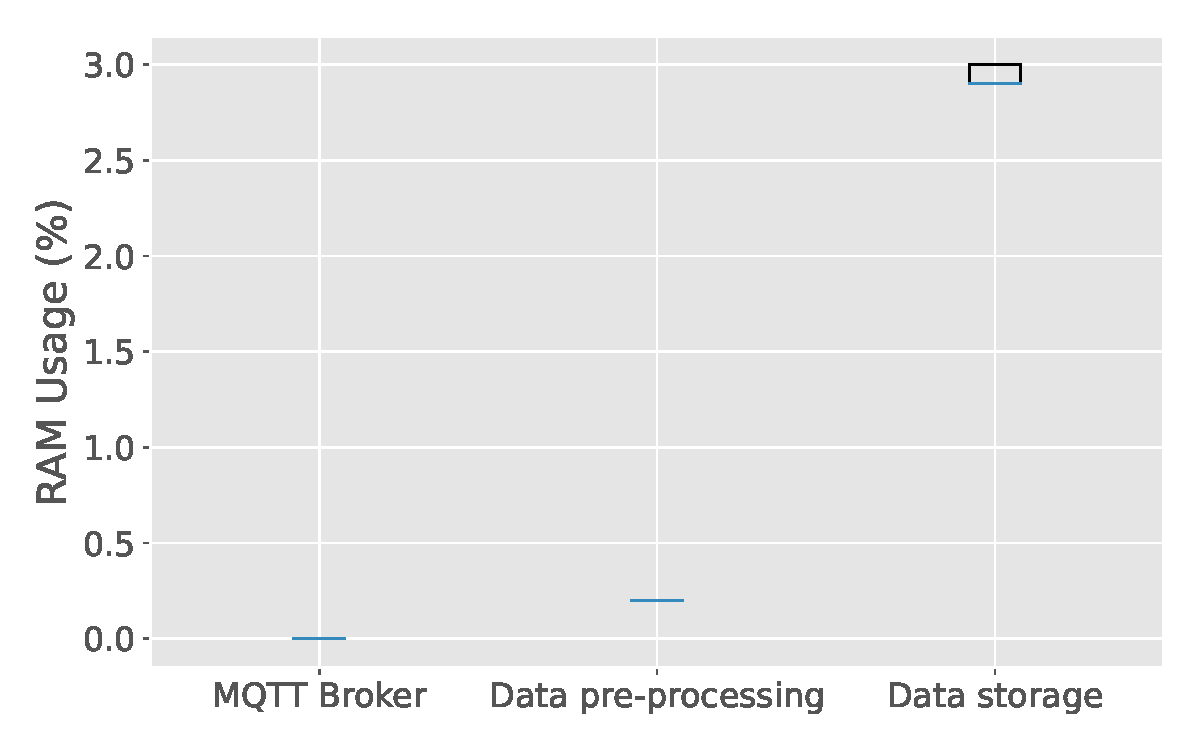
\includegraphics[width=\linewidth]{images/labtest_ram_usage_without_plugin.pdf}
        \caption{Average \acs{RAM} usage of each \textit{Smart Gateway} service measured over time during the lab tests, without using the custom plugin for Mosquitto.}
        \label{fig:labtest-ram-usage-noplug}
    \end{minipage}
\end{figure}


\begin{figure}[H]
    \begin{minipage}{0.45\linewidth}
        \centering
        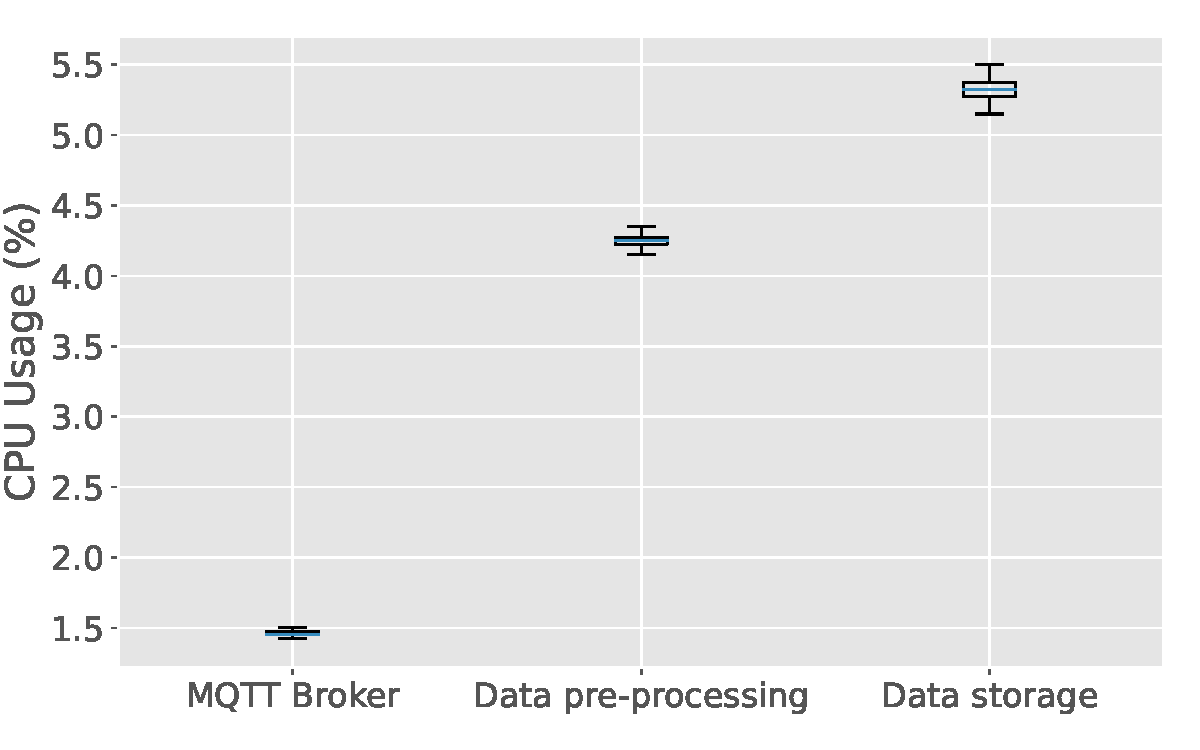
\includegraphics[width=\linewidth]{images/labtest_cpu_usage_with_plugin.pdf}
        \caption{Average \acs{CPU} usage of each \textit{Smart Gateway} service measured over time during the lab tests, when using the custom plugin for Mosquitto.}
        \label{fig:labtest-cpu-usage}
    \end{minipage}
    \hspace{0.05\linewidth}
    \begin{minipage}{0.45\linewidth}
        \centering
        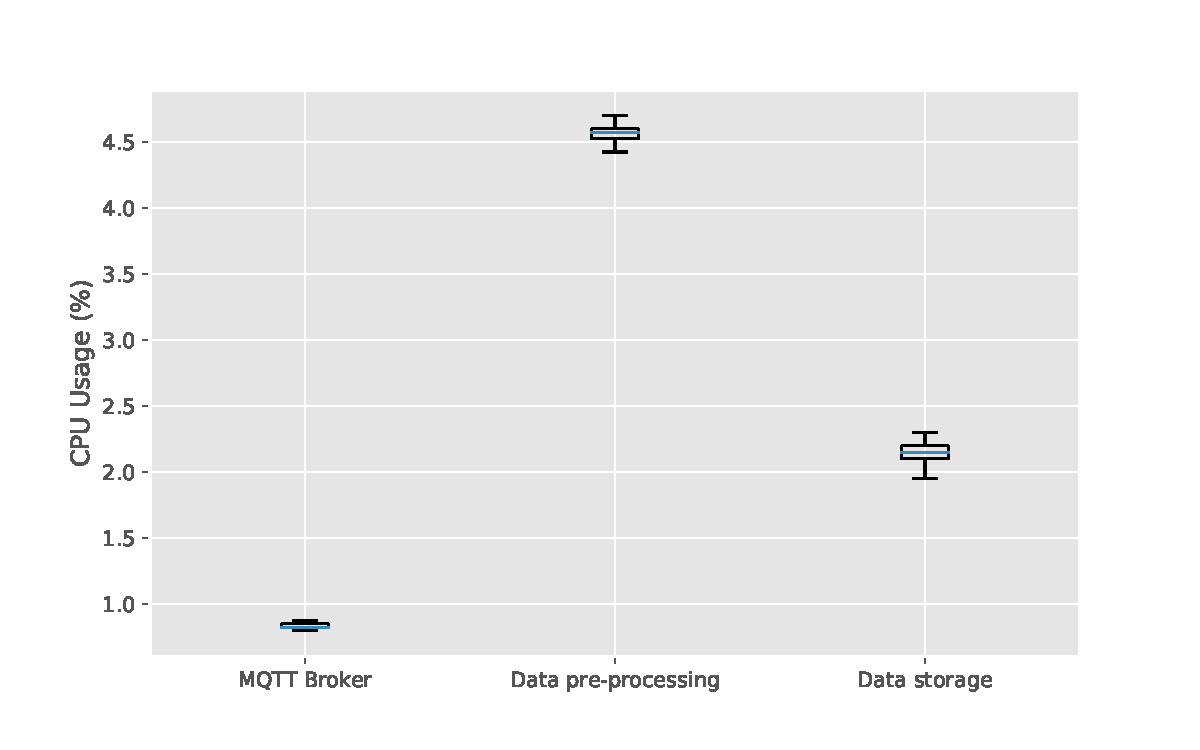
\includegraphics[width=\linewidth]{images/labtest_cpu_usage_without_plugin.pdf}
        \caption{Average \acs{CPU} usage of each \textit{Smart Gateway} service measured over time, without using the custom plugin for Mosquitto.}
        \label{fig:labtest-cpu-usage-noplug}
    \end{minipage}
\end{figure}

\paragraph{} Overall, the results reported are extremely positive, since they demonstrate the performance of the system developed throughout this past year. Certain phenomena should be researched further, for example the observed latency deviations on \acs{MQTT} communications, but nonetheless, the developed architecture should provide a solid foundation for the ongoing development of the \acs{WoW} project.

\section{Summary}
In this chapter, the performance of the proposed system has been experimentally evaluated and discussed. 
In the next, and final chapter, an overview of the work achieved is presented in light of the proposed contributions, concluding with some final remarks.